\section{Mercato del lavoro}
\subsection{Evoluzione del mercato del lavoro}
Nel dossier tematico “Nuove forme di lavoro per un mondo in continua evoluzione” elaborato dalla Camera di Commercio si evidenzia un cambiamento nella cultura del lavoro scaturito dall’introduzione delle nuove tecnologie e che ha portato alla diversificazione produttiva, alla flessibilità e al just in time. Cambiamento che è stato favorito dalla globalizzazione e dalla diffusione delle nuove tecnologie dell’informazione e della comunicazione che hanno permesso l’interconnessione di mercati mondiali delle merci e dei capitali, delle idee, delle competenze e della professionalità. Questi fattori hanno spinto la capacità d’innovazione, la competitività e la concorrenza internazionale a livelli sempre più alti, stimolando le aziende ad evolvere. Sull’onda della quarta rivoluzione industriale si è innestata la nuova economia digitale, che sta trasformando la produzione di beni e servizi, la loro distribuzione e gli stili di vita delle persone. I cambiamenti produttivi e sociali modificano inevitabilmente i modelli di lavoro: termini come lavoro alternativo, immateriale, telelavoro, job sharing, ecc. sono sempre più correnti. La gig economy (lavoro “on demand”) e la sharing economy (economia della condivisione) hanno ampliato e diversificato l’offerta di merci e servizi, allargando anche la base occupazionale grazie alla rapidità dell’incontro tra domanda e offerta di lavoro. Questa situazione ha portato un aumento degli impieghi a tempo parziale che rappresenta una vera e propria svolta dal punto di vista sociale per l’opportunità che dà alle persone inattive sul mercato del lavoro da tempo come casalinghe, disoccupati e giovani che stanno studiando, di entrare a farvi parte; dal punto di vista strettamente legato ai cambiamenti della quarta rivoluzione industriale, il part-time potrebbe permettere alle aziende di assumere un maggior numero di impiegati a percentuale ridotta sapendo di poter contare sulla produttività e l’efficienza dei robot e delle intelligenze artificiali che garantirebbero un maggior profitto.
\subsection{Nuovi modelli del mercato del lavoro}
Nel dossier vengono inoltre riportati i risultati di un recente studio europeo (Eurofound) che ha classificato nove grandi tipologie di nuovi modelli di lavoro diffusi in tutto l’Occidente:
\begin{itemize}
    \item Employee sharing: gli stessi lavoratori vengono assunti da un gruppo di diverse imprese.
    \item Job sharing: il lavoro viene ripartito tra più dipendenti.
    \item Temporary management: manager impiegati per specifici progetti.
    \item Casual work: lavoro intermittente.
    \item Telelavoro: lavoro da casa.
    \item Voucher-based work: le prestazioni vengono pagate con un voucher che copre retribuzione e contributi sociali.
    \item Portfolio work: freelance che lavorano per diversi clienti.
    \item Crowd employment: piattaforme online che mettono in contatto domanda e offerta di lavoro per progetti complessi.
    \item Collaborative employment: lavoratori indipendenti e micro imprese che collaborano tra di loro.
\end{itemize}
Si tratta di modalità di impiego che sono nate dalle trasformazioni economiche e sociali odierne e che le aziende dovrebbero sempre più adottare per aumentare l’innovazione. In generale le condizioni di lavoro flessibili costituiscono un vantaggio concorrenziale decisivo e possono trarne beneficio sia i datori di lavoro sia i dipendenti. Queste forme di lavoro permettono non soltanto di migliorare la conciliabilità di vita professionale e vita privata migliorando la qualità di vita dei collaboratori, ma anche di pianificare con intelligenza il lavoro.

\subsection{Il mercato del lavoro nella quarta rivoluzione industriale}
Questa situazione è oggi e sarà sempre più la realtà che la quarta rivoluzione industriale sta realizzando; una realtà che richiederà da una parte una nuova cultura del lavoro e dall’altra impone l’impegno comune della politica, delle parti sociali e delle aziende. Solo così e pensando alla realizzazione di modelli più efficienti di Welfare e di modelli aziendali molto diversi rispetto a quelli tradizionali si potranno affrontare le sfide delle grandi trasformazioni della quarta rivoluzione industriale. La formazione continua, la previdenza professionale, la mobilità e la discontinuità lavorativa, l’accesso all’impiego per i più giovani saranno concetti chiave della trasformazione e dei cambiamenti da apportare al sistema attuale.
\subsection{Composizione attuale del mercato del lavoro}
Secondo il documento “Ai margini del mercato del lavoro”, il mercato ticinese, così come quello nazionale, è fortemente terziarizzato. Sul nostro territorio, il settore dei servizi offre il 70.9% dei posti di lavoro (media nazionale è del 71.2%). Altri settori che offrono un numero importante d’impieghi sono le attività manifatturiere, il commercio (all’ingrosso e al dettaglio), le costruzioni e la sanità e assistenza sociale. L’economia ticinese si differenzia nei rami dove la quota di addetti ETP (impieghi a tempo pieno) è superiore a quella nazionale, ovvero nelle costruzioni (Ticino 10.9%, Svizzera 8.2%), nel commercio (Ticino 15.4%, Svizzera 13.4%), nel finanziario (Ticino 6.4%, Svizzera 5.8%) e nei servizi di alloggio e di ristorazione (Ticino 5.3%, Svizzera 4.8%).
\begin{figure}
    \centering
    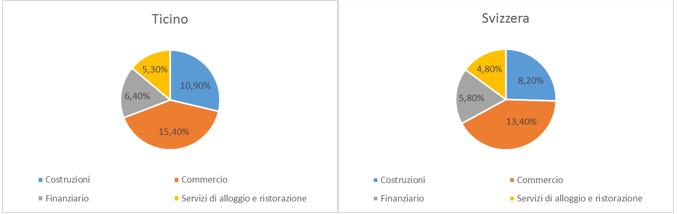
\includegraphics{Grafico settore terziario.PNG}
    \caption{Caption}
    \label{Composizione settore terziario in Ticino e Svizzera}
\end{figure}
\textbf{In sintesi} l’economia ticinese rappresenta in termini di aziende e addetti tra il 4% e il 5% di quella nazionale, inoltre negli ultimi anni l’economia ticinese è cresciuta a un ritmo più sostenuto di quella nazionale. In Ticino, come nel resto del paese, il tessuto economico è prevalentemente costituito da micro-imprese con meno di 10 addetti ETP. L’economia ticinese è molto terziarizzata e i rami di specializzazione (rispetto a quelli elvetici) sono le costruzioni, i comparti turistici, i rami del finanziario e del commercio.
Negli ultimi anni l’occupazione in Ticino ha subito una crescita, anche se comunque quasi la metà degli occupati sul territorio è di nazionalità straniera. Si è verificato un aumento degli impieghi a tempo parziale a causa dell’evoluzione che il mercato del lavoro sta vivendo e diventa sempre più esigente la richiesta di profili qualificati.
Per quanto riguarda i salari in Ticino crescono moderatamente e generalmente in tutti i segmenti della popolazione. Tenuto conto delle differenze professionali e personali dei lavoratori, permangono ancora importanti differenze salariali a sfavore delle donne rispetto agli uomini e dei frontalieri rispetto a svizzeri e stranieri residenti.
